\documentclass[conference]{IEEEtran}
\IEEEoverridecommandlockouts

\usepackage{amsmath,amssymb,amsfonts}
\usepackage{algorithmic}
\usepackage{graphicx}
\usepackage{textcomp}
\usepackage{xcolor}
\usepackage[numbers]{natbib}
\usepackage{graphicx}

\usepackage{todonotes}
\newcommand{\cit}[1][]{\todo[tickmarkheight=0.2cm]{cit #1}}

\begin{document}

\title{Explainable AI and cognitive bias: opportunities and perils of AI explanation}

% \title{Trusting explanations: what can we expect from XAI?}

\author{\IEEEauthorblockN{Alvise de' Faveri Tron}
    \IEEEauthorblockA{\textit{Politecnico di Milano} \\
        alvise.defaveri@mail.polimi.it}}

\maketitle

\begin{abstract}
    Artificial Intelligence (AI) has become an increasingly significant part of
    our societies and private lives nowadays. From curation systems that can
    influence what we buy, what we watch, what we believe in and who we vote
    for, to systems that can decide who to hire, predict criminal recidivism,
    and operate on the stock market, many fields have adopted some kind of AI
    system for tasks that would normally require human intelligence. However,
    this kind of technology is known to suffer from interpretability problems:
    it is often hard for humans to understand why an AI-based system took a
    particular decision and to identify the general logic behind an AI's
    behavior. XAI (short for eXplainable AI) is a research field that aims at
    finding methods to explain these machines' behaviors or individual decisions
    in a way that is intelligible to humans. Although there are great
    opportunities in this field, there is also a risk associated to the creation
    of intermediate explanation layers. Human decision-making is in fact known
    to be affected by cognitive bias, for instance the so-called \textit{framing
        effect}, which happens when our decisions are influenced by the way
    information is presented. This paper wants to explore how explanation
    systems could, in principle, leverage decision-making biases to convince
    human operators that their internal model is correct, or present decisions
    in a way that they are not questioned, if these explanation interfaces are
    not cautiously evaluated.
\end{abstract}

%-----------------------------------------------------------------%
\section{Introduction}
\label{sec:intro}

Artificial Intelligence is an umbrella term that is commonly used to describe a
multitude of technologies and approaches. While a precise definition of this
term involves many complex aspects, such as defining the meaning of intelligence
and its relation with human thinking (\citet{Norvig}, chapter 1.1), in this
paper I want to focus on those computing techniques that are currently used to
take automated decisions in complex situations, i.e. in which the desired
behavior cannot be easily synthesized using simple rules.

One of such techniques is Machine Learning, which has enabled many of the recent
advances in the field. It is used to recognize handwritten digits, people and
objects in pictures, translate from one language to another, drive cars, and
suggest photos, videos and posts on platforms such as Facebook and YouTube.

While, on one hand, these techniques have achieved incredible results, and the
surrounding technology has become mature enough to be employed in fields such as
medicine, law and finance, on the other hand there is a lot of research that has
highlighted the social, cultural and political implications of some of the
side-effects of ML-based systems, for example when they learn biased models or
spurious correlations.

Yet, most of the popular top-performing algorithms in use today, such as Deep
Convolutional Neural Networks (DCNNs), Genetic Algorithms, Swarm Intelligence
and Statistical Machine Learning in general, are known to be difficult to
examine and understand for humans.

Most of these algorithms are in fact built to reason in a statistical way, are
composed of a large number of elements (e.g. neurons in DCNNs) and can have very
complex structures.

This aspect represents a huge technical and ethical issue for this field,
especially when building autonomous systems that are meant to replace or aid
humans in highly impacting decisions. If we can't explain "why" a certain
algorithm took a certain decision, how can we trust these systems? How do we
ensure that their internal models are not biased or broken? How do we understand
when the machine is failing?

The problem of introspection and accountability for these systems is a very
serious one. Marvin Minsky et al. raised the issue that AI can function as a
form of surveillance, with the biases inherent in surveillance, suggesting HI
(Humanistic Intelligence) as a way to create a more fair and balanced
``human-in-the-loop'' AI. \citet{minsky}.

As a natural result of these emerging concerns about AI, the field of
Explainable AI (XAI) was born. The goal of this research field is to build
systems that can provide humans with a deeper understanding of AI algorithms,
with the ultimate objective of making errors and biases more easy to spot or
predict and AI-based systems generally more trustworthy.

Yet, because of the young age of this field and because of the intrinsic
complexity of the problem, there is still a lack of definition of what
\textit{explainable} means, and there is a somewhat confused terminology around
the idea of \textit{interpretability}.

In this paper, I want to analyze some of the extreme consequences of the lack of
such definition, and more generally the lack of a comprehensive way to evaluate
AI explanations.

Since there is no widely accepted way of evaluating explanations, each
researcher tends to focus on one or just a few aspects of interpretability.
\citet{Giannotti} in particular shows that many studies concentrate on the
\textit{complexity} of the explanation. I want to show in this paper that an
evaluation system based solely on how easy it is to understand an explanation,
without taking into account aspects such as fidelity, might produce potentially
harmful explanation interfaces.

In particular, I want to show that the presence of well known cognitive bias in
the way humans understand and accept explanations can distort the evaluation of
these explanations, and if this aspect is not taken into account, AI explanation
could amplify the problem of unconscious biases in technology instead of
mitigating it.

To explain this idea, I will proceed as follows:

In Section~\ref{sec:background}, I will provide some background on the problems
which XAI is trying to solve and a classification of the solutions that are
currently being developed.

In Section~\ref{sec:explainability}, I will introduce the problem of defining
interpretability, and propose a classification of the aspects that define an
explanation.

In Section~\ref{sec:troubles}, I will discuss the idea that explanation
interfaces might be able to fool a human user into believing that a specific
algorithm is doing the right thing, leveraging his or her own bias.

Finally, Section~\ref{sec:counterarg} contains a list of possible critiques to
the ideas expressed in this paper and Section~\ref{sec:conclusions} contains
some concluding thoughts on this subject.

%-----------------------------------------------------------------%
\section{Background}
\label{sec:background}

\subsection{Current issues of AI}
\label{sec:opaque}

As AI has become more popular, there has been a vast number of studies on
potential or actual negative externalities of real-world AI systems. One
well-known category is curation and filtering algorithms for online platforms
and search engines, for example YouTube.

\citet{tufekci2018youtube} claims that ``Youtube may be one of the most powerful
radicalizing instruments of the 21st century'', and automated suggestions play a
key role in this, since 70\% of the videos watched are recommended by an
ML-based system  \citet{solsman}.

\citet{epstein} found that biased search engine results can shift the voting
preference of undecided voters by 20\%.

Challenges such as fake news, biased predictions and filter bubbles make the
understanding of ML-base curation systems an important and timely concern, but
there are even more sensitive contexts where defects in AI systems can provoke
disastrous consequences.

Some recent studies have shown how subtly gender, race and social biases can be
inherited by ML algorithms: facial recognition is known to have biases with
respect to skin color \citet{buolamwini2018gender}, Amazon's hiring algorithm
was shown to disproportionally prefer men to women \citet{hiring}, and the
COMPAS algorithm used to estimate criminal recidivism has been accused of racial
bias \citet{compas}.
% Also, removing racial or gender information from datasets is not a solution to
% this kind of problems, as there are other proxies to race, gender and social
% status that can equally inferred by statistical approaches.

More generally, we know that current AI is prone to what are called ``Clever
Hans moments'': a notorious example is \citet{cleverhans}, where the classifier
taken into consideration had learned to recognize image of horses because there
was a copyright tag that was present in about one-fifth of the horse figures in
the training dataset.

This goes to show that, despite the advanced results that have been achieved
with AI and Machine Learning, there are still many problems that require the
creation of introspection and explanation tools in this field.

% Modern complex AI techniques, such as deep learning and genetic algorithms,
% are naturally opaque \cit [24], yet they constitute the foundations of today's
% image and speech recognition, natural language processing, autonomous driving
% and many other intelligent systems. These are the kind of algorithms which are
% being considered in this paper.

% As this technology advances, we are starting to see the problems that derive
% from its opacity. In the 2010s public concerns about racial and other bias in
% the use of AI for criminal sentencing decisions and findings of
% creditworthiness have led to increased demand for transparent artificial
% intelligence. \cit [1] As a result, many academics and organizations are
% developing tools to help detect bias in their systems. \cit [22]

% Marvin Minsky et al. raised the issue that AI can function as a form of
% surveillance, with the biases inherent in surveillance, suggesting HI
% (Humanistic Intelligence) as a way to create a more fair and balanced
% ``human-in-the-loop'' AI. \cit[23]

% From a practical point of view, modern AI has been found to be particularly
% vulnerable to ``Clever Hans'' situations, in which an AI chooses the right
% answer for the wrong reason.

% It is important to notice that the problems highlighted in the above examples
% cannot be associated to any programming error of these systems, but is more of
% an inherent issues of these machines.

%-----------------------------------------------------------------%
% goals (introspection, human-in-the-loop, right for an explanation) scope
% (local vs global) techniques

\subsection{The XAI approach}
\label{sec:xai}

The term \textit{Explainable AI} refers to methods and techniques in the
application of artificial intelligence that aim at improving the possibility for
humans to understand AI algorithms. We can consider \citet{DARPA} as a starting
point for modern XAI research. Figure~\ref{fig:xai} reports the goals of XAI as
stated in that paper. The idea is that we want to be able to better understand
when a given AI-based system is doing something wrong, when we can trust it and
why an error occurred. All these aspects contribute to improving
\textit{accountability}, since who makes use of such systems can and must verify
their behavior, \textit{transparency}, since the reasons for a certain decisions
are in theory stated in an understandable way, and \textit{fairness}, since
understanding the reasons enables us to oppose a certain decision.

\begin{figure}[h!] 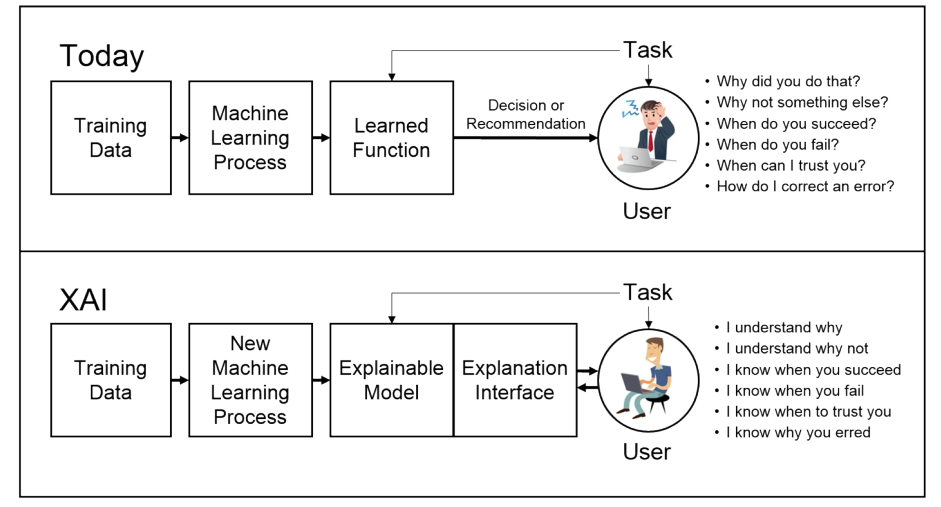
\includegraphics[width=\linewidth]{images/xai.png}
    \caption{The goals of XAI as expressed in \citet{DARPA}. } \label{fig:xai}
\end{figure}

\subsection{Proposed Solutions}
\label{sec:solutions}

% \citet{Giannotti} proposes the following high-level classification for XAI
% techniques, as shown in Figure~\ref{fig:xaiclass}:

% \begin{itemize} \item \textit{Model explanation}: Global explanation of the
%     whole model's behavior. \item \textit{Outcome explanation}: Local
%     explanation of a single outcome. \item \textit{Model inspection}:
%     Explanation trough introspection of the model's internals. \item
%     \textit{Transparent Box design}: Making AI easier to understand by design,
%     e.g. by using algorithms that are intrinsically clearer for humans.
%     \end{itemize}

% \begin{figure}[h!] 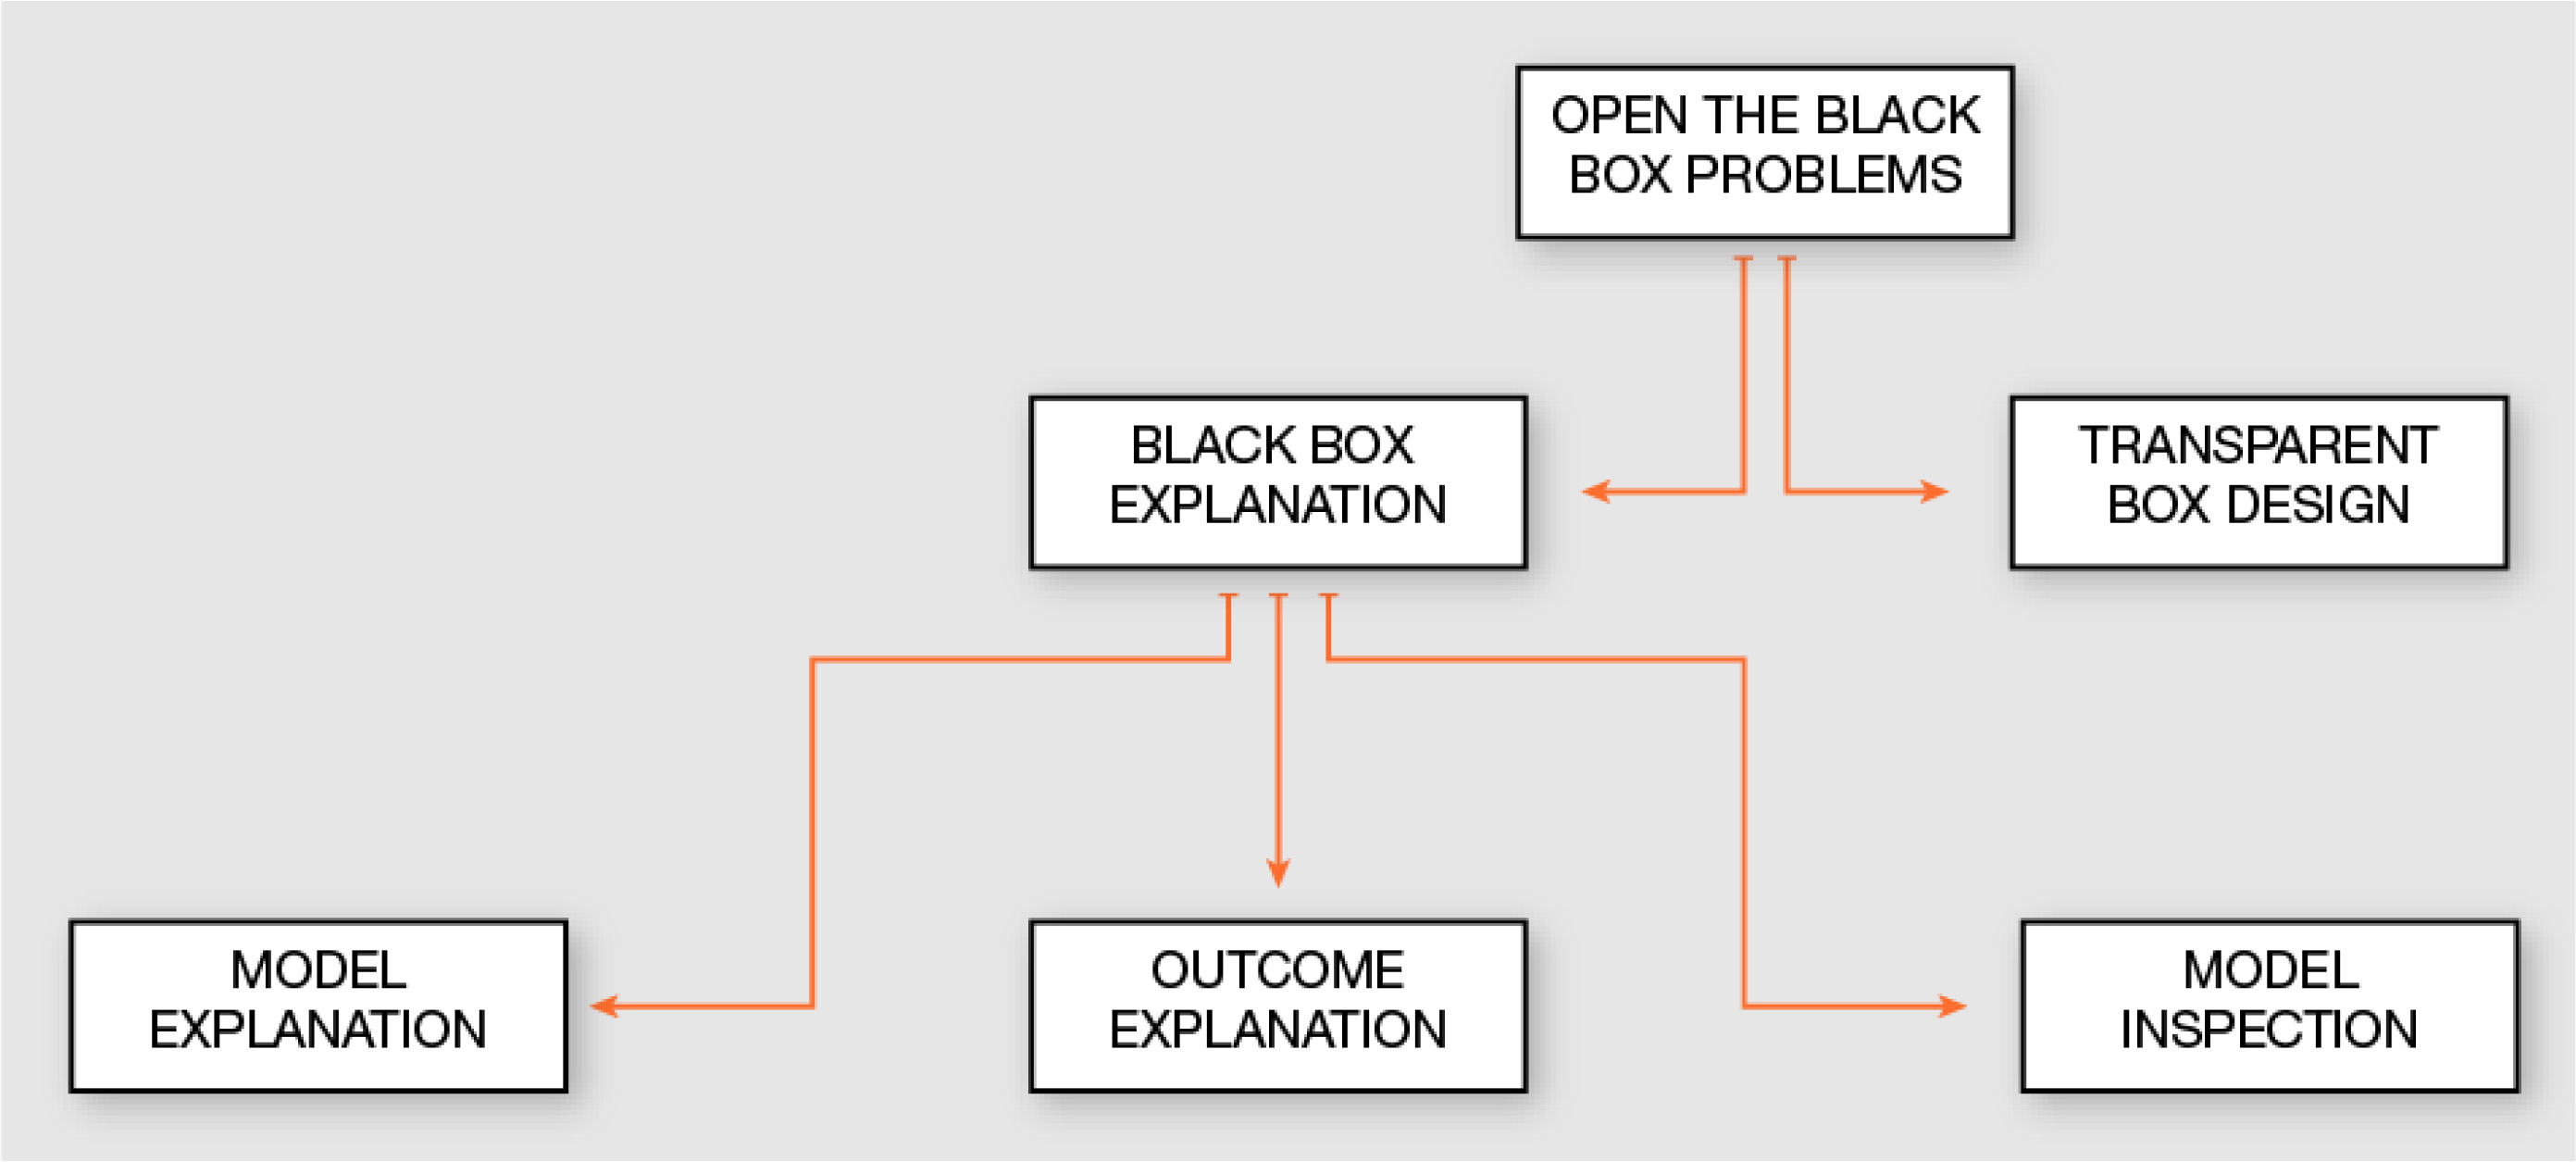
\includegraphics[width=\linewidth]{images/xaiclass.png}
%     \caption{Taxonomy of XAI solutions provided by \citet{Giannotti}}
%     \label{fig:xaiclass} \end{figure}

From a general perspective, \citet{Giannotti} identifies two families of
approaches to this problem: \textit{transparent box design}, which aims at
building algorithms that are more explainable by design, and
\textit{reverse-engineering} approaches, also called \textit{post-hoc
    interpretability} approaches, which try to provide explanations for already
existing algorithms.

Some examples of the latter type are listed in \citet{nasaxai}.

\textit{Visualization}, for example, focuses on finding visual representations
of key aspects of the model, for example using \textit{saliency masks} as shown
in Figure~\ref{fig:heatmap}.

\begin{figure}[h!] \centering
    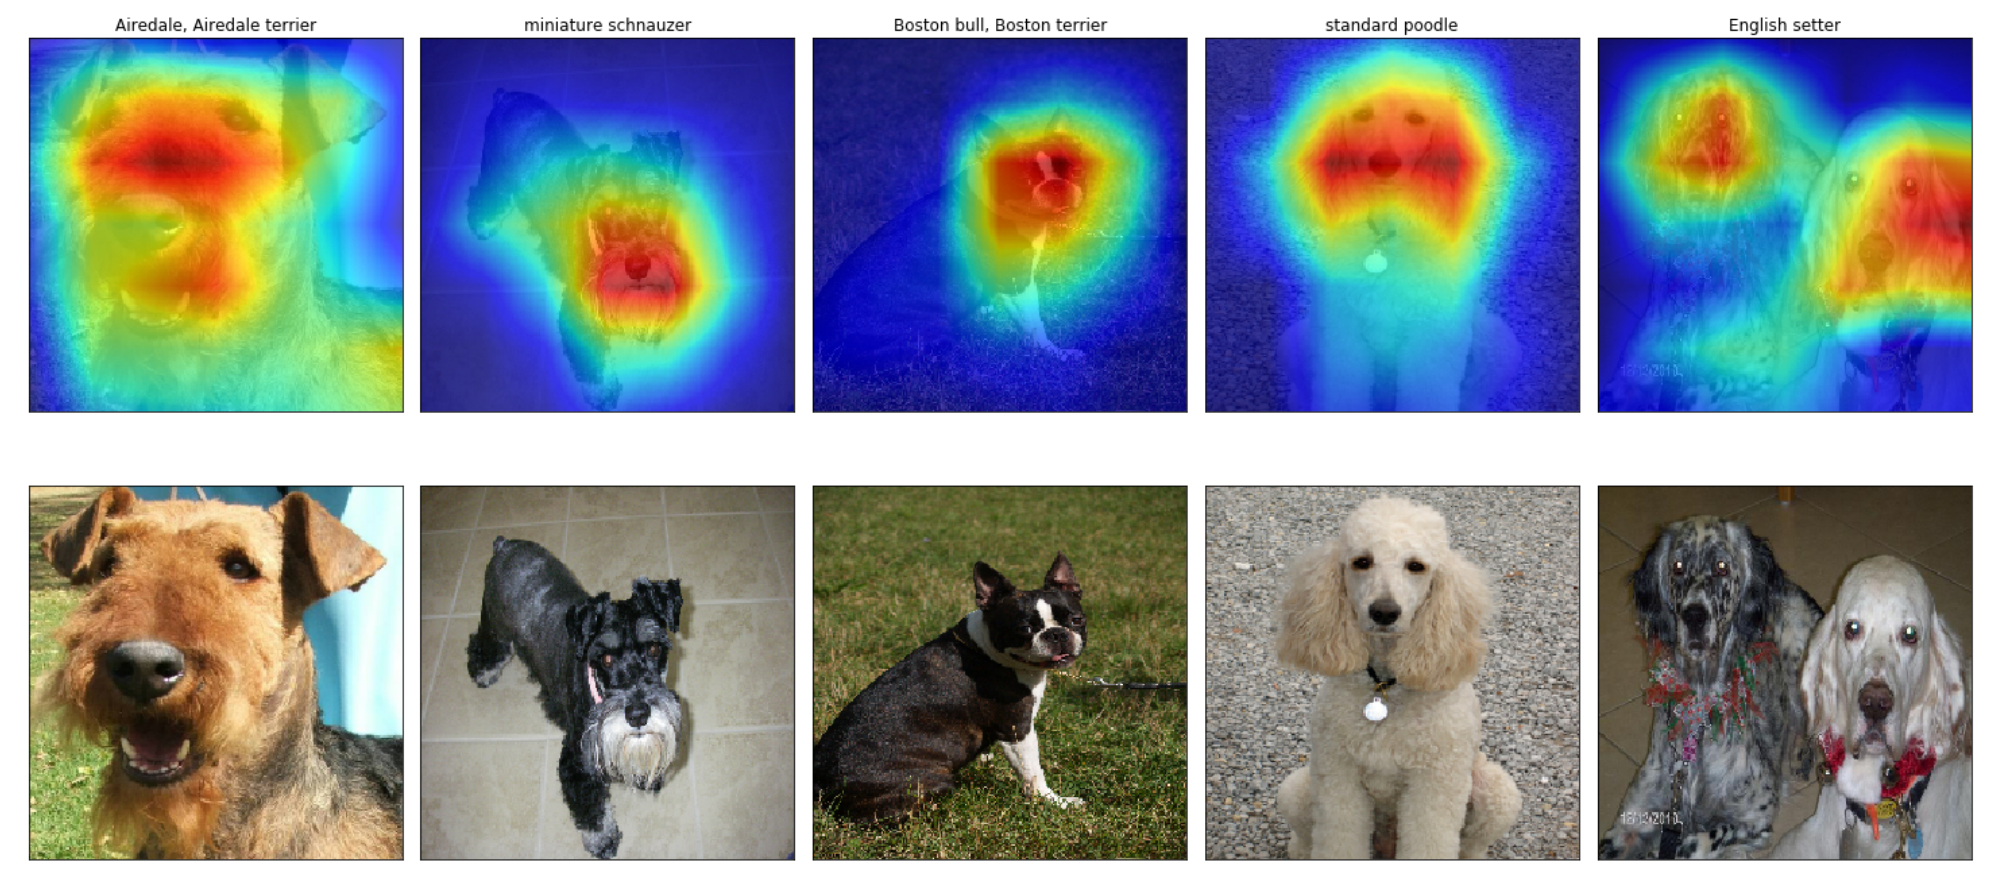
\includegraphics[width=0.9\linewidth]{images/dog_localization.png}
    \caption{An example of a heatmap representing the importance of each pixel
        in determining if a picture has been classified as containing a dog, from
        blue (low importance) to red (high importance). } \label{fig:heatmap}
\end{figure}

\textit{Approximation} consists in using simple models or simplifying already
existing models: in \textit{single tree approximation}, for example, the
internal structure of an AI algorithm is approximated to a classification tree,
shown in Figure~\ref{fig:dectree}.

\begin{figure}[ht!] \centering
    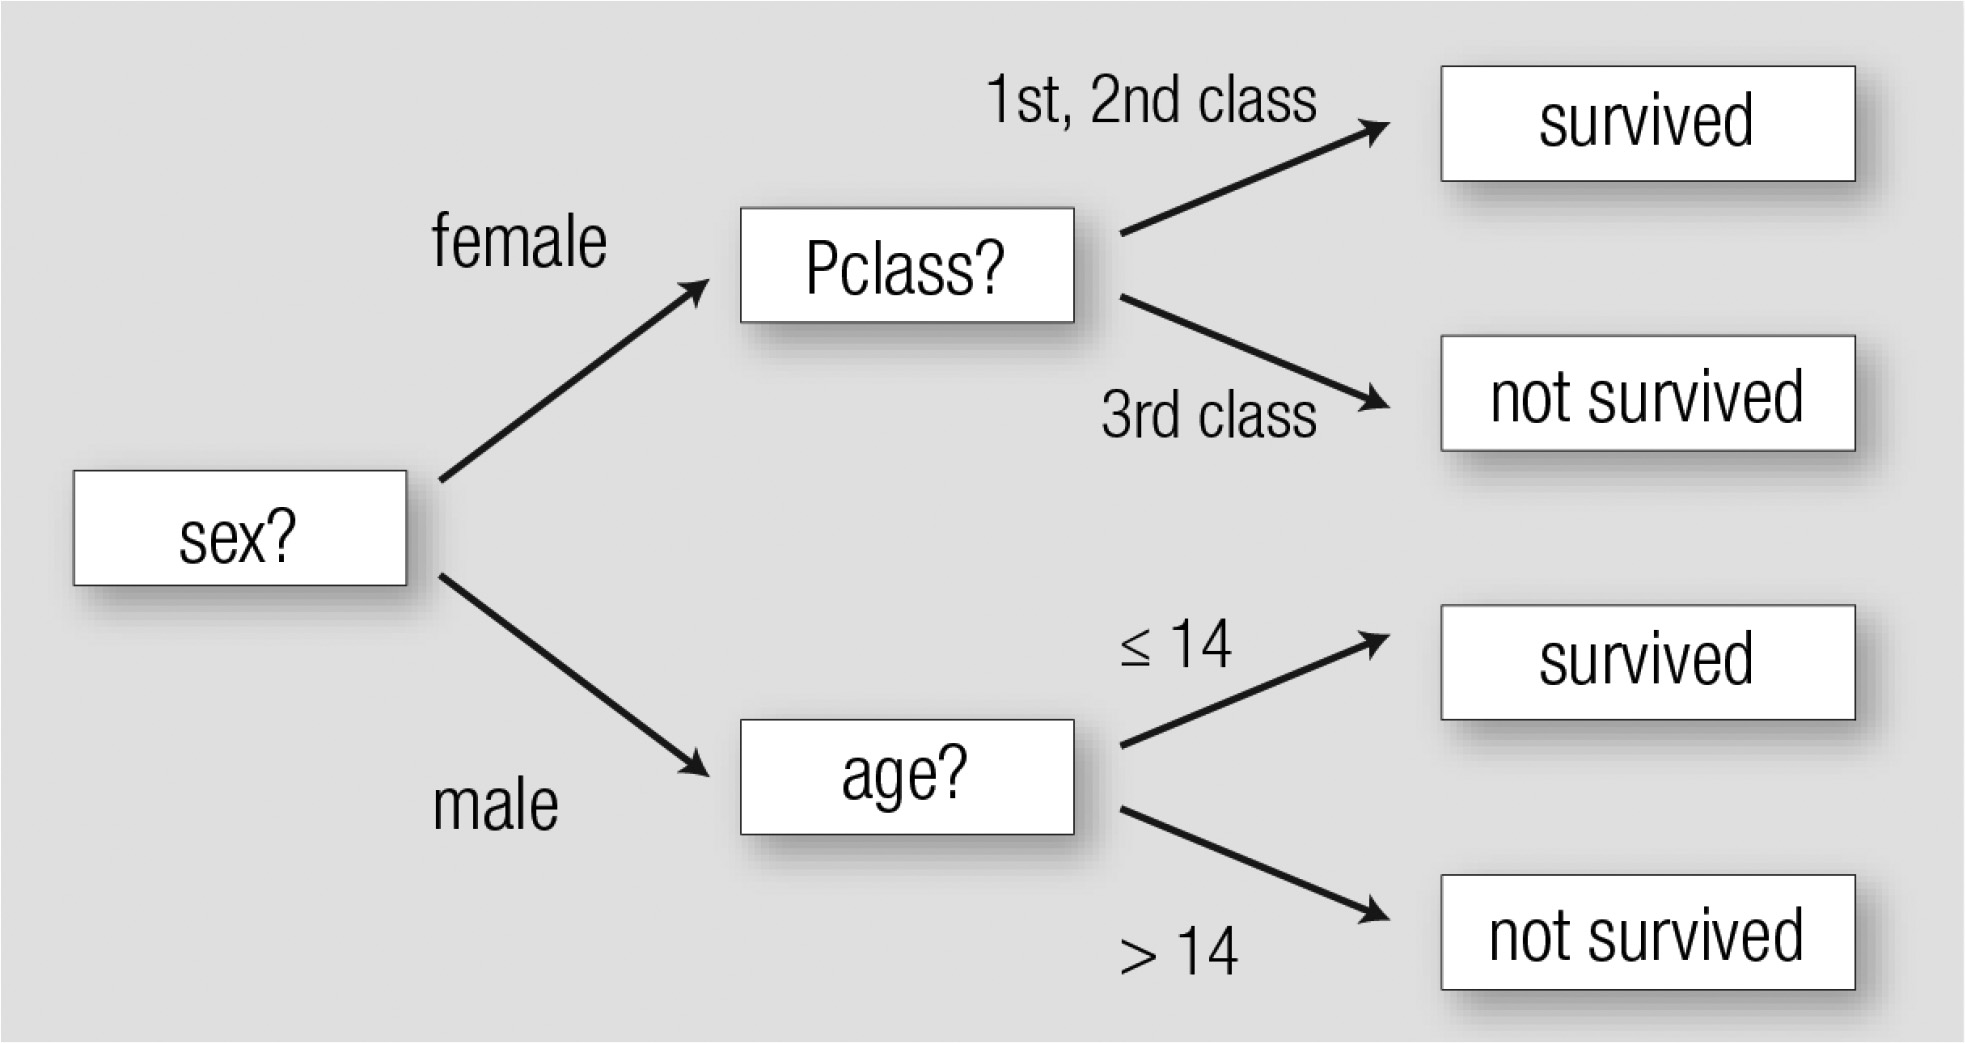
\includegraphics[width=0.9\linewidth]{images/dectree} \caption{A simple
        Decision Tree} \label{fig:dectree} \end{figure}

\textit{Causal Models (CAMEL)} try to generate causal explanations of Machine
Learning operations and present them to the user as intuitive narratives.
% A scheme of the architecture needed for this approach is illustrated in
% Figure~\ref{fig:camel}.

% \begin{figure}[ht!] \centering
%     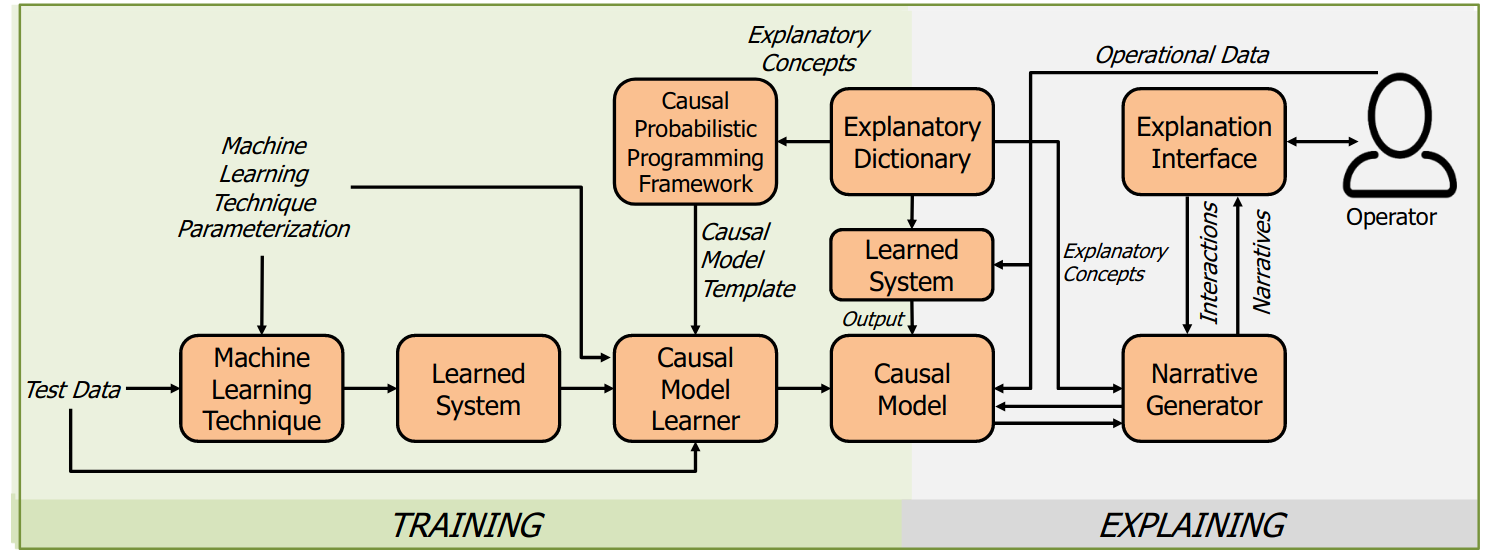
\includegraphics[width=0.9\linewidth]{images/camel.png}
%     \caption{Architecture of the CAMEL approach.} \label{fig:camel}
%     \end{figure}

Other approaches include \textit{Learning and Communicating Explainable
    Representations}, where explanations themselves are learned as a separate
part of the training process, and \textit{Explanation by Example}, where the
AI is able to provide an example, or a \textit{prototype}, of how it thinks
that a typical member of a given class should appear and/or which
characteristics should be changed to change the outcome.

% It is quite clear that each approach carries a very different notion of what
% is an explanation: some focus on representing specific properties of the
% model, while other try to create a more abstract way of describing the model's
% behavior.

It is important to notice how different approaches produce explanations that
have different \textit{distances} from the original model: for example, in some
sense we can say that visualization is a quite ``close'' representation of the
AI's internal model, since it represents how the internal neurons are activated,
while in techniques such as CAMEL and Learned Explanations there is a much more
indirect connection between elements of the original model and elements of the
explanation, which is also expression of the increased complexity of the
interface itself.

This intuitive idea of \textit{distance} will be further explored in
Section~\ref{sec:fidelity}.

%-----------------------------------------------------------------%
\section{Defining Interpretability}
\label{sec:explainability}

\subsection{Dimensions of AI Explanation}
\label{sec:dim}

As anticipated in Section~\ref{sec:intro}, one fundamental problem in the field
of XAI is that there is no single conventional notion of interpretability.
\citet{mythos} goes as far as considering the term itself ill-defined, therefore
stating that claims about interpretability generally have a quasi-scientific
nature. \citet{Giannotti} on the other hand, considers the lack of a
mathematical description as an obstacle for the future development of this
field. \citet{DARPA} itself defines the formalization of an evaluation metric
for explanations as one of the goals of the XAI program, to be developed in
parallel with technical solutions.

When analyzing the problem of defining and evaluating interpretability, two
questions naturally arise:

\textbf{Explainable to whom?} The concept of \textit{user} of an AI system is
not always well defined, nor is the concept of user of an explanation. This
might include:

\begin{itemize}
    \item The \textit{developer} of the AI system, as he is only partially in
          control of what the algorithm does
    \item The \textit{operator} of an AI system: many AI algorithms nowadays are
          being used as an input for a human to make decisions on a certain
          subject
    \item The \textit{end user} which is affected by the decision of an AI
\end{itemize}

\textbf{Explainable for which purpose?} Different users have different needs,
which may partially overlap. Therefore there is a variety of goals that
explanations try to accomplish, and some of them might be in contrast with each
other. Some of these needs are:
\begin{itemize}
    \item \textit{Debugging}: finding errors and backtracking them to a specific
          reason
    \item \textit{Human-in-the-loop}: creating systems where human and AI
          decisions can co-exist and influence each other
    \item \textit{Validation}: understanding if a certain model is good enough
          to be deployed for a certain task
    \item \textit{Failure Prediction}: understanding which are the weaknesses of
          an AI system and when it is likely to fail
    \item \textit{Appeal AI decisions}: \footnote{This goal is not explicitly
              listed in the original scope of XAI, but has gained traction
              recently with the introduction of the concept of \textit{right for
                  an explanation} in Europe's new GDPR. (\citet{righttoexpl})}
          giving the right to users and citizens that are affected by AI
          decisions to know, understand and possibly appeal decisions that
          are automated with AI systems
\end{itemize}

It appears quite evident that different XAI solutions built with different users
in mind will have very different notions of what a good explanation is.

\subsection{Possible Metrics}
\label{sec:dimensions}

Bearing in mind the different goals that an XAI system can have, we can identify
a series of characteristics that are different among different solutions:

\begin{itemize}
    \item \textit{Complexity}: how many elements are there in the explanation?
    \item \textit{Clearness}: how cognitively hard is the explanation? How
          difficult is it to understand the correspondence between the elements
          of the explanation and the information we are trying to gain?
    \item \textit{Informativeness}: how much information, weighted on how
          meaningful is is, can be extracted by the explanation? E.g. does the
          explanation significantly modify the level of uncertainty about the AI
          behavior?
    \item \textit{Fidelity}: how closely does the explanation represent the
          functioning of the system? Are all the facts inferred from the
          explanation also applicable to the original system?
\end{itemize}

Clearly, a specific metric will be more or less important depending on the
specific user and use-case. There is however a deeper distinction that has to be
made, which is related to how these metrics are measured.

Complexity, for instance, is often measured using a quantifiable proxy, such as
the number of elements in the explanation, which can be for example the depth of
the decision tree or the number of neurons. On the other hand, clearness and
informativeness are more difficult to quantify a-priori, but could be
empirically evaluated by providing the explanations to a group of people and
verifying how they respond.

In general, we can identify two ways of evaluating an AI explanation: one is
using a direct measurement of some quantity that we can derive directly from the
explanation. The second one is considering an explanation itself a black-box,
and check if it actually provides a better understanding of the AI model to some
selected group of individuals used as a benchmark. While the first method is not
always feasible, since choosing which quantity is representative of a certain
aspect is in itself a difficult decision to make, the second method clearly
presents the same problems of opaqueness and unreliability that AI models
themselves have.


%-----------------------------------------------------------------%
\section{The troubles of explanations}
\label{sec:troubles}

\subsection{Measuring fidelity}
\label{sec:fidelity}

Of all the metrics highlighted in Section~\ref{sec:dimensions}, fidelity, also
called \textit{faithfulness} in literature (\citet{explainingexpl}) , is
probably the most complex to evaluate. On one hand, the maximum fidelity is
already represented by the implementation itself, but on the other hand the
reason we need explanations is that the implementation itself is not clear
enough.

This is particularly important since AI explanations are also targeted to
unspecialized users, which need to understand what's happening without
necessarily having a solid background on the internal functioning of such
systems.

Yet, fidelity plays a fundamental role when we have to evaluate an AI algorithm,
as it quantifies the difference between what is being evaluated (the AI model)
and the instrument we are using for this evaluation (the AI explanation). This
is what we intuitively defined as \textit{distance} between the model and the
explanation in Section~\ref{sec:solutions}, and represents in some sense the
``measurement error'' introduced by the explanation.

% Let's take for example the situation depicted in Figure~\ref{fig:eval}: in
% this case, a human operator is evaluating an AI model trough an explanation
% interface.

% \begin{figure}[h!] \centering
%     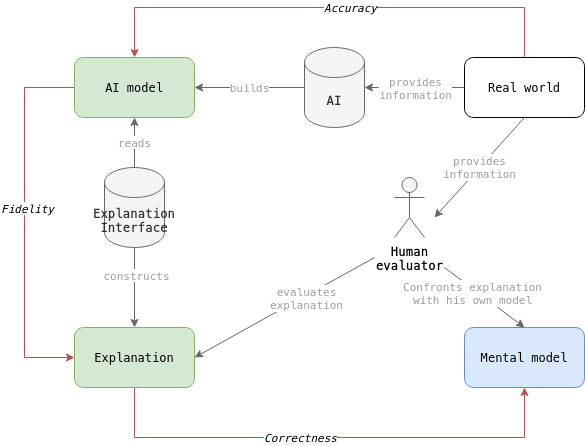
\includegraphics[width=0.9\linewidth]{images/evaluation.png}
%     \caption{Evaluation process of an AI through an explanation interfaces.}
%     \label{fig:eval} \end{figure}

While this idea might seem easy enough to understand, devising an operational
way to measure it is a non-trivial task.

Let's take for example Causal Models: in this case, the explanation and the
original model will typically have a very different nature, since the
explanation interface produces causal relationships, while the AI model
typically reasons in terms of statistical correlation. In this case, how can we
measure the fidelity of this interface?

On the other hand, being unable to measure fidelity poses another question: if
both the AI and the explanation are treated as black boxes, how can we be sure
that evaluating the AI using that explanation interface will effectively improve
our understanding of the underlying AI model? Couldn't it be that we just
\textit{think} we understand it?

\subsection{Decision making biases}
\label{sec:bias}

Human decision-making is known to be affected by many cognitive bias, which are
deeply rooted in our thinking and are often difficult, if not impossible, to
exclude when we make decisions. Recently, \citet{framingeffect} studied the
consequences of the \textit{framing effect} in the domain of AI, in particular
how likely is a person to accept or reject an AI recommendation based on how the
output was framed. An interesting result of this research is, for example, that
``\textit{perceived reasonableness was significantly higher when the suggestion
    of AI was provided before the decision is made than after the decision is made
    when perceived accuracy was controlled}'' (\citet{framingeffect}, page 5).

While this is not a direct study on AI explanation interfaces, it does show how
the same local decision of an AI can be judged differently just varying the
timing of the explanation, and a similar result has been found when looking to
how the solution is framed (positive or negative sentences etc.).

This goes to show how the evaluation of the correctness of an AI model is not
only a subjective matter, but can vary in the same individual depending on
factors that are external to the AI behavior itself.

\subsection{Can explanation interfaces learn to exploit cognitive bias?}
\label{sec:exploit}

As a pure thought experiment, let's imagine a situation where a single
individual is in charge of deciding whether an explanation interface is suited
for understanding a certain type of AI architecture, e.g. Neural Networks, and
let's make the assumption that the only observable elements are the output of
the AI model and the explanation provided by the interface. This settings is not
far from the one of an operator who acts upon AI recommendations.

Let's then suppose that the explanation interface is a complex interface that
can convert the model's internals into a human-like reasoning, for example by
producing textual motivations for a certain output.

As shown in Section~\ref{sec:bias}, it is completely possible that the judgment
about the correctness of the algorithm is biased by the way the explanation
interface presents the information. Let's now suppose that the same individual
has to select,  between multiple explanation interfaces and multiple AI models,
the best couple of model-explainer to be put in production: even if the single
explanation interface is not built to learn from the individual's taste, this
environment creates a selection for those explanation systems that present
information in a way that is perceived better by the operator.

Although in the ideal case this leads to selecting an explainer that is clear
and comprehensible for a human, a possible outcome could also be selecting a
couple in which the explainer is very convincing at justifying the AI model. In
absence of other information, the individual has equal probability of selecting
the most correct explanation interface and the most accurate AI model, or the
most convincing explanation interface coupled with a sub-optimal model.

This scenario effectively describes a situation in which we have created an
explanation machine which is so good at producing convincing explanations that
it could also \textit{lie} without being detected.


%-----------------------------------------------------------------%
\section{Counterarguments}
\label{sec:counterarg}

% critiques:
% 1. allora non si può fare niente per migliorare l'interpretabilità?
% 2. le AI mica hanno lo scopo di fotterti
% 3. c'è lo stesso problema con ogni rappresentazione allora
% 4. si può fixare se valuti quanto la spiegazione incrementa la predittività sì
%           ma c'è sempre il problema del test set vs vita reale

Some criticisms that can be made to this argument are:

\begin{itemize}
    \item \textit{Can't the problem stated in \ref{sec:exploit} be overcome by
              simply adding more judges?} While this is true, the problem of cognitive
          bias is that it can also be inherited from the group or society around the
          single individual. Certainly, a diverse control group for evaluating
          explanations is a must-have, but it is not a complete guarantee of absence
          of bias.
    \item \textit{Can't errors introduced by the explanation interface be simply
              corrected by looking at the actual behavior of the AI?} If the explanation
          interface behaves like a black-box, there is the same problem that affects
          AI testing in general: even if testing is done extensively and all results
          are positive, i.e. the explanation is always perfectly aligned to the AI
          model, we have no general guarantee that this holds for all the possible
          outcomes.
    \item \textit{Can't we just use explanations that have a high fidelity with
              respect to the AI model?} While this is a possible solution when the
          explanation is used for debugging purposes, we should not forget that the
          audience of AI explanation is much broader, and it is especially important
          that non-expert people that are subjected to the decisions of an AI system
          are given the possibility to understand them.
\end{itemize}

%-----------------------------------------------------------------%
\section{Conclusions}
\label{sec:conclusions}

In conclusion, we have shown how the fact that there is no single definition of
what interpretability is and no comprehensive way of evaluating simultaneously
all the important aspects that compose an explanation, especially fidelity,
leads to the possibility of creating yet another black-box layer over the
black-box model, which can accentuate biases instead of reducing them.

While the proposed argument is just a thought experiment, there are many
realistic elements in this setting that should warn us about the possibility of
creating deceitful explanation interfaces.

The goal of this paper is not to discourage the research in the field of XAI,
which is essential for the advance of AI in general, but to show how complex and
multi-faceted the problem of AI explanation is.

\bibliographystyle{plainnat}
\bibliography{references}

\end{document}
